%% ==============================
\chapter{State of the Art}
\label{sec:state_of_the_art}
%% ==============================
The following overview of the state of the art consists of four main parts:
\begin{enumerate}
    \item The general theory of path planning in mobile robotics is presented. This includes the most common algorithms for path planning and their applications in real robotic systems. (Chapter \ref{sec:path_planning}).
    \item The recent approaches to hierarchical path planning in complex multi-floor environments are presented. This shows the existing approaches to the first research question: "How to navigate in complex multi-floor environments?" (Chapter \ref{sec:hierarchical_planning}).
    \item The recent approaches to straight path planning are presented. This shows the existing approaches to the second research question: "How to plan paths that are straight and predictable?" (Chapter \ref{sec:straight_paths}).
    \item The research gap and limitations of the state of the art are summarized in Chapter \ref{sec:research_gap}.
\end{enumerate}

%% ==============================
\section{General Path Planning for Mobile Robots}
\label{sec:path_planning}
%% ==============================
The general approach to path planning in mobile robotics is a two-layered architecture, as shown in Figure \ref{fig:path_planning_two_layered_architecture}. The first layer is the global path planning layer. It is responsible for finding a path from the start to the goal position in a previously known static environment. The second layer is the collision avoidance layer, also known as the local path planner or controller. It is responsible for avoiding dynamic obstacles that prevent the global path from being executed. For both layers there are different approaches available as open source solutions. This concept is further explained with the example in the Chapter \ref{sec:navigation_stack}.

\begin{figure}[h]
    \centering \captionsetup{justification=centering}
    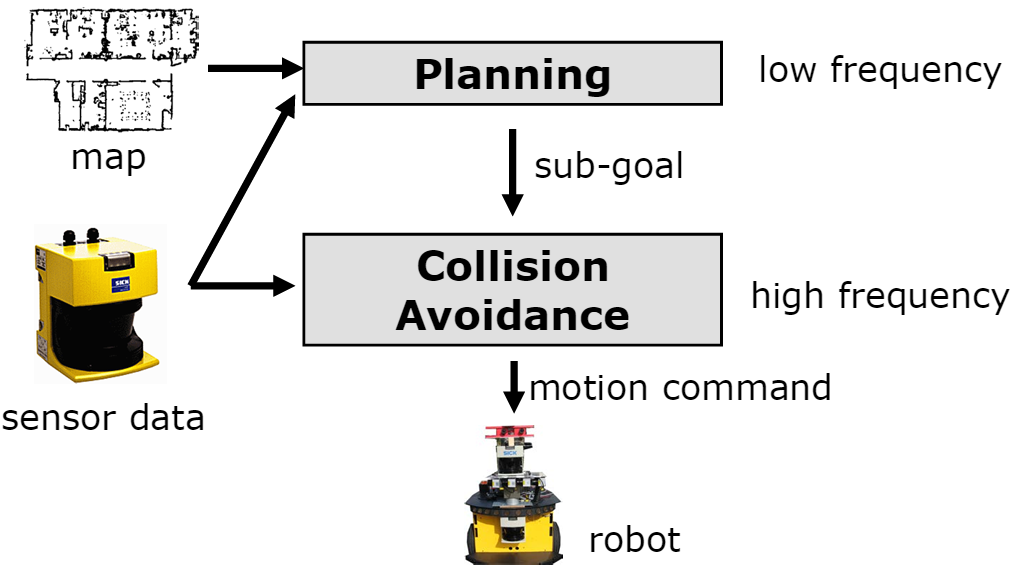
\includegraphics[width=0.75\textwidth]{figures/20_state_of_the_art/path_planning_two_layered_architecture.png}
    \caption[The two-layered architecture for mobile robot path planning]{The two-layered architecture for mobile robot path planning (Source: \cite{burgard_introduction_2021})}
    \label{fig:path_planning_two_layered_architecture}
\end{figure}

The scope of this work is limited to extending the capabilities of the global planner to multiple floors. Collision avoidance is solved using existing algorithms. The following sections provide an overview of the most common existing global planner algorithms. 

%% ==============================
\subsection{Path Planning Algorithms}
Path planning is a major challenge in robotics and is necessary for mobility. The path from the robot's current location to the goal can be planned in two ways: deterministically or probabilistically. Deterministic planners use algorithms that always produce the same results given the same input. Probabilistic planners, on the other hand, rely on randomness and produce different results for the same input. The map on which deterministic planners are based is usually discretized into a lattice. In an informed search, heuristics can be used to determine whether one grid cell is closer to the target configuration than another. According to Burgard et al. \cite{burgard_introduction_2021}, the performance of a search algorithm is measured in four different ways:
\begin{enumerate}
    \item Completeness:
    Does the algorithm find a solution when there is one?
    \item Optimality:
    Is the solution the best one of all possible solutions in terms of path cost?
    \item Time complexity:
    How long does it take to find a solution?
    \item Space complexity:
    How much memory is needed to perform the search?
\end{enumerate}

Among the deterministic planners, there are several prominent representatives, such as the Dijkstra algorithm or the A* algorithm as a special form of it. A* was originally proposed by Hart et al. \cite{hart_formal_1968} and is widely used in research. A* plans a path from the start configuration to the target configuration. During expansion, each new node is evaluated with the metric \ref{equ:metric}. 
\begin{equation} \label{equ:metric}
    f(n) = g(n) + h(n)
\end{equation}
The node with the lowest metric value is expanded next. The metric consists of the cost of the previously traveled path \(g(n)\) to the current node \(n\) plus the estimated cost of the remaining path to the destination \(h(n)\). This estimate is computed using a heuristic such as the Euclidean distance or Manhattan distance for gridmaps. It is important that the heuristic never overestimates the real cost to ensure the optimality of the A* algorithm. In planar 2D space, there is no path shorter than the direct line with the length of the Euclidean distance. The expansion is performed until the target node is part of the expanded nodes. The shortest path is then traced by following the parent nodes back to the start.

The Dijkstra algorithm \cite{dijkstra_note_1959} is a generalized form of A* and only considers the previous cost \(g(n)\) during the expansion. In general, this leads to more nodes being searched and a longer search time for the goal than A*. The time and space complexity of Dijkstra is higher than that of A*. Both algorithms have the advantage of providing complete and optimal solutions.

\begin{figure}[h]
    \centering
    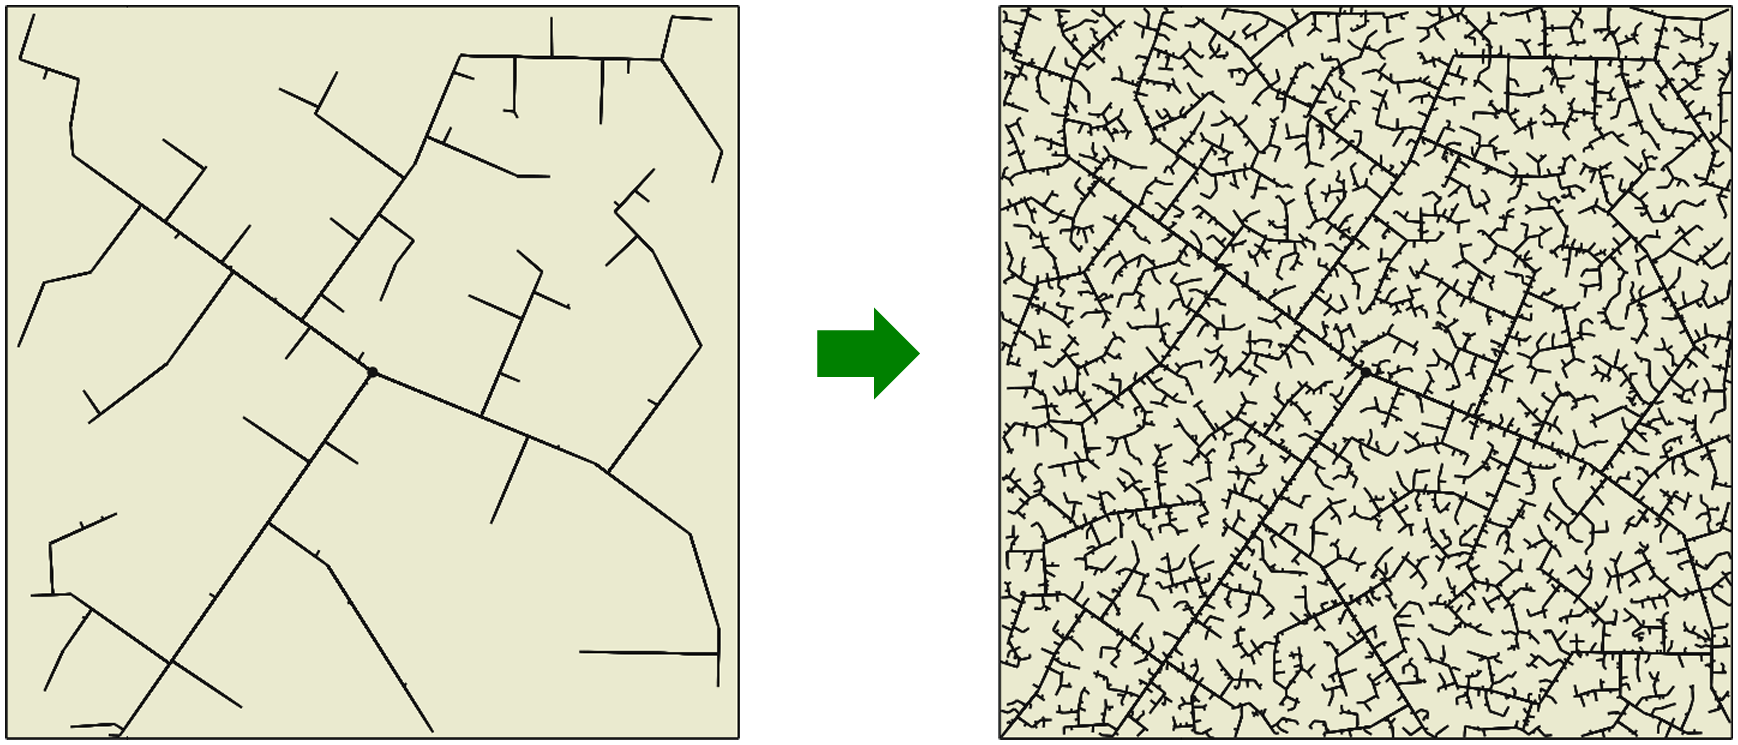
\includegraphics[width=1\textwidth]{figures/20_state_of_the_art/rrt.png}
    \caption[The RRT algorithm]{Rapidly Exploring Random Tree (RRT) after 45 (left) and 2345 (right) iterations from the starting node in each center. (Source: \cite{burgard_introduction_2021})}
    \label{fig:rrt}
\end{figure}

Unlike deterministic planners, probabilistic planners are based on the principle of randomness. One example among many is the RRT. New nodes are randomly selected in the search area, and then an attempt is made to connect them to the nearest node that is already part of the tree. This connection must meet two conditions: First, there is no obstacle in the direct connecting line, and second, the distance to the tree is not greater than \(d_{max}\). If the first criterion fails, the selected node is discarded. If only the second criterion fails, a new node is created on the link with the distance \(d_{max}\) and added to the tree. This procedure produces large trees after only a few iterations, as can be seen in Figure 2.3. With an appropriately chosen \(d_{max}\), this method needs significantly fewer nodes to reach the goal than an A*. In addition, as the number of nodes approaches infinity, this algorithm also moves in the direction of completeness, but this method is not optimal. Time and memory complexity depend on \(d_{max}\).


%% ==============================
\subsection{The Robot Operating System 2}
\begin{displayquote}
    \enquote{The \acrfull{ros} is a framework for writing robot software. It is a collection of tools, libraries, and conventions that aim to simplify the task of creating
    complex and robust robot behavior across a wide variety of robotic platforms.} (Source: Quigley et al. \cite{quigley_programming_2015})
\end{displayquote}
    
\begin{figure}[h]
    \centering
    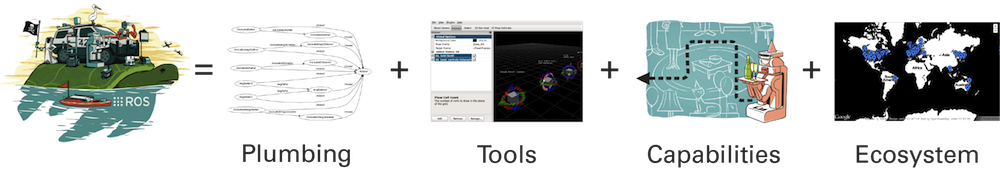
\includegraphics[width=1\textwidth]{figures/20_state_of_the_art/ros_equation.png}
    \caption[The ROS equation]{The ROS equation: ROS = Plumbing + Tools + Capabilities + Community (Source: \cite{open_robotics_ros_2020})}
    \label{fig:ros_equation}
\end{figure}

Development of \gls{ros} began in 2007 as part of the Stanford AI Robot Project (STAIR) and was primarily driven by Willow Garage. It was used there as the basis for the Personal Robot 2 (PR2), but was intended from the start as an open source platform for a wide range of robotic applications. Development is now being driven by Open Robotics. Its founders, Brian Gerkey and Morgan Quigley, have also published a comprehensive book to facilitate entry into \gls{ros} \cite{quigley_programming_2015}. The \gls{ros} ecosystem consists of much more than just code; it thrives on a large community and the sharing of ready-to-use packages, which is described by the "\gls{ros} equation" in the Figure \ref{fig:ros_equation}. Since 2011, \gls{ros} has left Earth for the International Space Station with NASA's Robonaut 2 \cite{koubaa_ros_2016}. Due to the rapidly growing community and increasing use in industry, an improved version was developed and released in December 2018 as \gls{ros_2}. The main difference is the focus on real-time applications and the use of the industry standard 'Data Distribution Service' (DDS) for communication of distributed systems \cite{macenski_robot_2022}.

Nodes are the basis of the distributed network of a \gls{ros} application. The nodes are executed independently and communicate with each other via defined interfaces. This has the advantage that applications can be built modularly, easily exchanged and used in conjunction with other applications. A node can contain several topics, services or actions that exchange data with other nodes. Different nodes in a \gls{ros} application can run on different hardware. A collection of nodes that perform a certain function are grouped together as a package and shared by many developers around the world. A combination of related packages with a version history and maintained documentation is called a stack. For example, there is the Navigation stack, which contains all the functions needed to get the robot safely from A to B. This includes algorithms for localization and path planning, as well as processing of sensor data for obstacle avoidance and mapping.
\begin{figure}[h]
    \centering
    \captionsetup{justification=centering}
    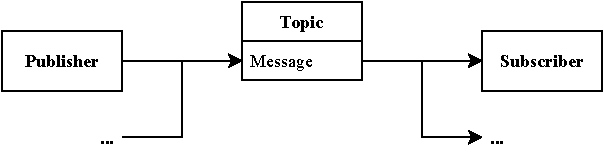
\includegraphics[width=0.75\textwidth]{figures/20_state_of_the_art/topics.pdf}
    \caption{The structure of a ROS topic}
    \label{fig:topics}
\end{figure}
The individual nodes communicate via message channels about a specific topic. This communication is designed for distributed systems and allows many-to-many (n:m) cardinality. This means that any node can act as a publisher or subscriber of any topic, see Figure \ref{fig:topics}. The content of the message is defined by a .msg file as an interface.
\begin{figure}[h]
    \centering
    \captionsetup{justification=centering}
    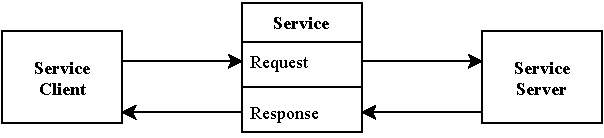
\includegraphics[width=0.75\textwidth]{figures/20_state_of_the_art/services.pdf}
    \caption{The structure of a ROS service}
    \label{fig:services}
\end{figure}
Services are based on a call-and-response model. This means that, unlike topics, messages are not sent unidirectionally across the network. Instead, a request is made from a client to a server and a response is sent back, as shown in Figure \ref{fig:services}. The structure is analogous to a function call, where parameters are passed and a return value is expected. The data types are defined in the corresponding .srv file. This type of communication is particularly useful for computations performed by another node \cite[p. 51]{quigley_programming_2015}. Services can be called synchronously or asynchronously. In a synchronous call, the calling node blocks the thread until the response arrives. Synchronous calls should only be used when the service requires a short, finite amount of time to compute. Asynchronous calls are implemented by providing a predefined function (callback) that is automatically invoked by \gls{ros} when the service response is received. This allows other code to be executed in the node as long as it does not depend on the service result.
\begin{figure}[h]
    \centering
    \captionsetup{justification=centering}
    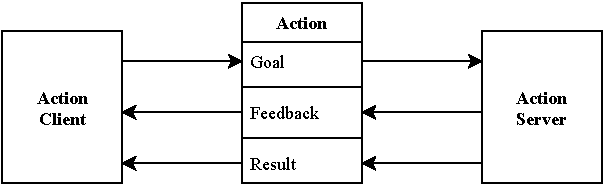
\includegraphics[width=0.75\textwidth]{figures/20_state_of_the_art/actions.pdf}
    \caption{The structure of a ROS action}
    \label{fig:actions}
\end{figure}
Actions have been an integral part of the communication vocabulary since \gls{ros_2}. They are designed for asynchronous execution of long-running actions. In addition to the concept of services, actions allow the exchange of feedback data during execution. Actions also provide the ability to abort their execution. An action client sends a request (goal) to the action server, which can either accept or reject the goal. During execution, a feedback callback is invoked at the client until the result is received and processed. Actions provide a high-level communication protocol, as shown in Figure \ref{fig:actions}. A good example of the use of actions is the movement of a robot towards a specific goal. The task should be asynchronous and can vary in duration. The feedback mechanism can provide information about the current position of the robot, and if the goal becomes outdated, the action can be cancelled. The interface of a navigation action is defined by a .action file, as shown in Algorithm \ref{lst:navigatetopose.action}.

\lstset{language=python, caption={NavigateToPose.action, definition of an action interface for navigation}, label={lst:navigatetopose.action}}
\begin{lstlisting}
# goal
geometry_msgs/PoseStamped pose
-%{}%-%{}%-
# result
std_msgs/Empty result
-%{}%-%{}%-
# feedback
geometry_msgs/PoseStamped current_pose
builtin_interfaces/Duration navigation_time
int16 number_of_recoveries
float32 distance_remaining
\end{lstlisting}
    
%% ==============================
\subsection{The Navigation Stack in ROS2}
\label{sec:navigation_stack}

\begin{displayquote}
    \enquote{Nav2 is the professionally supported spiritual successor of the ROS Navigation Stack. This project seeks to find a safe way to have a mobile robot move to complete complex tasks through many types of environments and classes of robot kinematics. Not only can it move from Point A to Point B, but it can have intermediary poses, and represent other types of tasks like object following and more. Nav2 is a production-grade and high-quality navigation framework trusted by 50+ companies worldwide.} (Source: Macenski \cite{steve_macenski_navigation_2020})
\end{displayquote}

\begin{figure}[!b]
    \centering \captionsetup{justification=centering}
    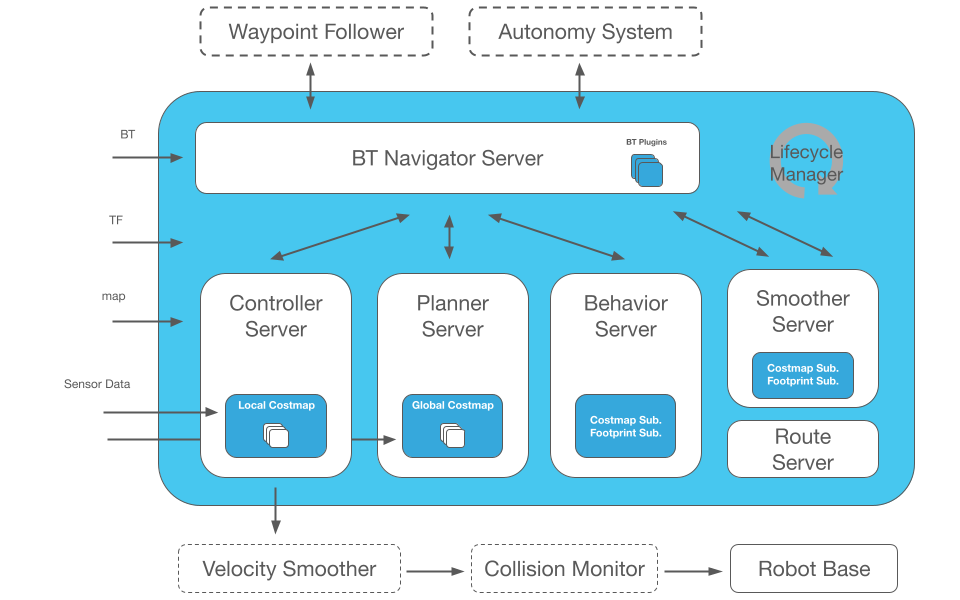
\includegraphics[width=\textwidth]{figures/20_state_of_the_art/nav2_architecture.png}
    \caption[The architecture of the Nav2 stack]{The architecture of the Nav2 stack (Source: \cite{steve_macenski_navigation_2020})}
    \label{fig:nav2_architecture}
\end{figure}

The \gls{nav_2} stack for \gls{ros_2} is a comprehensive framework for the development of new planner algorithms. The planner developed in this work is based on the \gls{nav_2} stack and is written as an exchangeable plugin for the existing structure. With its server and plugin layout, \gls{nav_2} supports custom planners, controller behavior, and smoother plugins. Figure \ref{fig:nav2_architecture} shows the architecture of \gls{nav_2}. It follows the classic two-layered path planning architecture shown in Figure \ref{fig:path_planning_two_layered_architecture}. The planner server provides the global path planning on a known map, and the controller server offers algorithms for following this path with dynamic obstacle avoidance. The necessary inputs for this system are the map, the odometry of the robot's wheels, and the sensor data from lidars or cameras. With this information, localization can calculate the most likely position of the robot on the map. The planner plans a path from this current position to the goal. In a control loop, the controller tries to reduce the error between the current position and the planned path. The output of the controller is a velocity command for the robot. The velocity command is then executed by the robot's motor controller.

In this work, a new planner is developed that is capable of planning in complex multi-floor environments. The algorithm is implemented as a plugin for the planner server. The rest of the \gls{nav_2} pipeline is used with existing packages.

%% ==============================
\subsection{Behavior Trees for Navigation}

\gls{nav_2} is the most prominent example of \glspl{bt} in robotics and specifically for navigation. It uses \glspl{bt} to create custom and intelligent navigation behavior by orchestrating many independent modular servers. The default \gls{bt} for executing a navigation request to a specific goal is shown in Figure \ref{fig:nav2_bt}. It shows the actual planner, an A* algorithm, on the left, which is triggered every second (1 Hz). All other named actions are recovery behaviors, which are used to clear the cost maps and reorient the robot if it gets stuck. To understand the symbolic language of the \gls{bt}, the individual elements are explained in the following section.

\begin{figure}[h]
    \centering \captionsetup{justification=centering}
    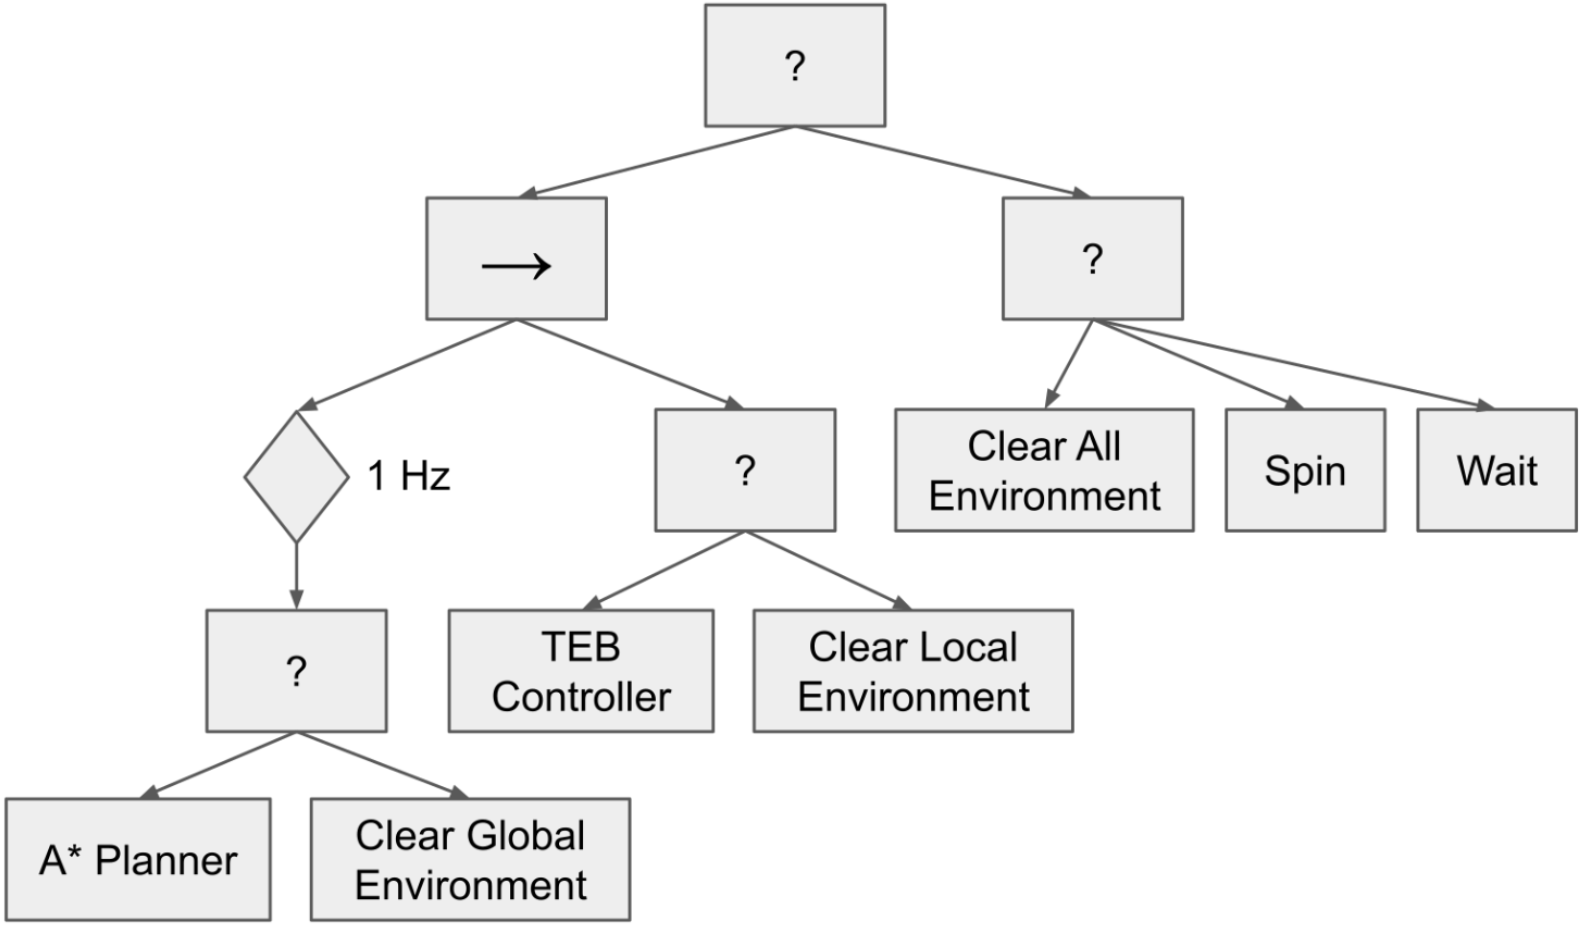
\includegraphics[width=\textwidth]{figures/20_state_of_the_art/nav2_bt.png}
    \caption[The default navigation behavior]{The default navigation behavior (Source: \cite{macenski_marathon_2020})}
    \label{fig:nav2_bt}
\end{figure}

\Glspl{bt} were developed for video games to describe the behavior of computer-controlled characters in a modular way \cite{hutchison_evolving_2010}. \Glspl{bt} combine a deliberative approach with reactive components. The internal structure of the tree defines an overall plan of action, ensuring goal-oriented behavior. However, reactive behavior can still be triggered through constant reevaluation of all conditions. A \gls{bt} consists of small building blocks that can be combined to create any control structure. The biggest difference to State Machines is that in \glspl{fsm} a state-dependent transition is triggered after a specific input. In \glspl{bt}, on the other hand, the entire structure is updated at regular, short time intervals and all conditions are re-evaluated. This allows arbitrary transitions to occur based on the appropriate preconditions, without having to explicitly define them.

\begin{figure}[h]
    \centering
    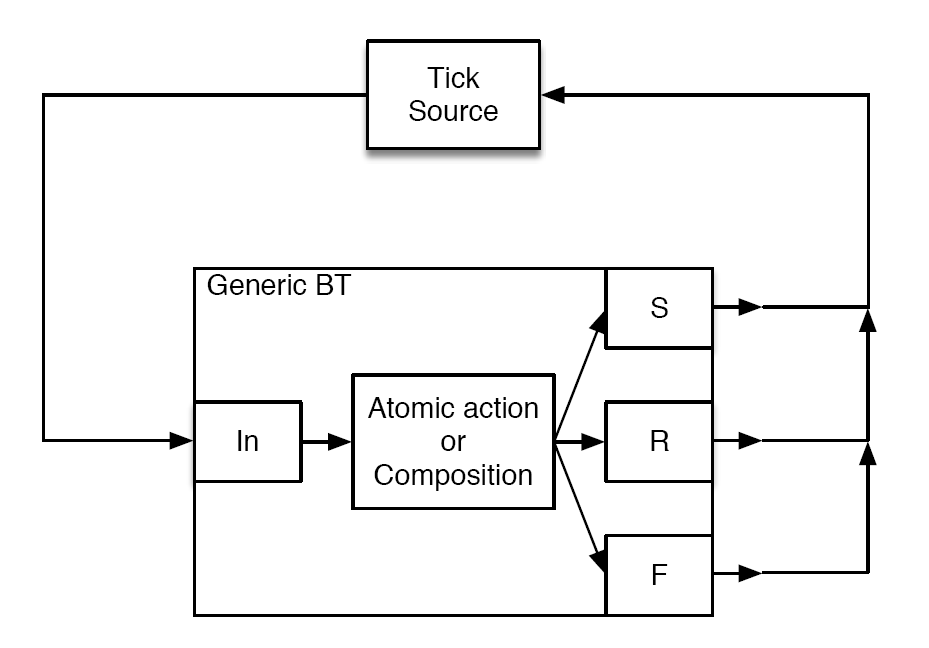
\includegraphics[width=0.7\textwidth]{figures/20_state_of_the_art/fsm_general_bt.png}
    \caption[General BT displayed as FSM]{General BT displayed as FSM with the state transitions: Success (S), Running (R) and Failure (F) (Source: \cite{colledanchise_behavior_2018})}
    \label{fig:fsm_general_bt}
\end{figure}

The fundamental element of every \gls{bt} is the root node, from which the attached nodes are updated (ticked). Each node returns either Success, Failure, or Running after being updated. In general, a \gls{bt} can be described using an \gls{fsm}, where the state transitions can take three possible states into account, as shown in Figure \ref{fig:fsm_general_bt}.

\begin{figure}[h]
    \centering \captionsetup{justification=centering}
    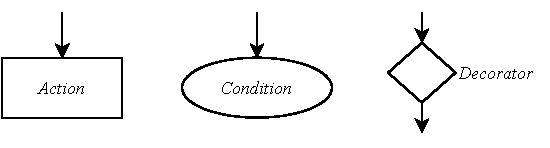
\includegraphics[width=0.7\textwidth]{figures/20_state_of_the_art/bt_types.pdf}
    \caption{Graphical representation of Actions, Conditions and Decorators}
    \label{fig:bt_types}
\end{figure}

The basic building blocks of a \gls{bt} are shown in Figure \ref{fig:bt_types}. Actions represent individual, self-contained algorithms that execute specific commands to actuators or perform calculations. An Action can run in a blocking (synchronous) manner, returning either Success or Failure after its start, or it can run asynchronously, maintaining a Running state during execution. Conditions, on the other hand, take either Success or Failure states depending on the condition being evaluated. The Decorator is a type of control node that has only one child. It allows the state of the child node to be influenced by custom rules, avoiding complex constructions with Sequences and Fallbacks. Examples of Decorators include Inverters, Time Delays, and Repeaters (repeating a certain number of times or until successful completion).

\begin{figure}[h]
    \centering \captionsetup{justification=centering}
    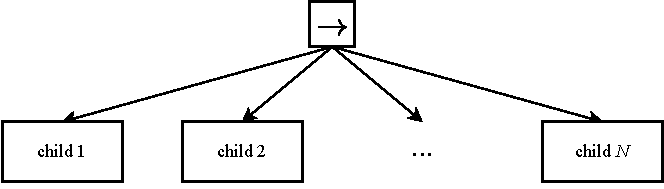
\includegraphics[width=0.75\textwidth]{figures/20_state_of_the_art/sequence.pdf}
    \caption{Graphical BT of a Sequence with \textit{N} childs}
    \label{fig:sequence}
\end{figure}

The Sequence starts its children from left to right in the graphical representation, as shown in Figure \ref{fig:sequence}. If a child returns Running, the entire Sequence is considered to be running. If a child executes successfully, the next child is started, and so on, until all children, and thus the entire Sequence, reach the state Success. If a child cannot be executed successfully, the loop is aborted and the Sequence enters the Failure state, as shown in Algorithm \ref{lst:pseudo_code_sequence}.
  
\lstset{language=C++, mathescape=true, caption={Algorithm of a Sequence with \textit{N} childs}, label={lst:pseudo_code_sequence}, morekeywords={from, to, is, do, then, end}}
\begin{lstlisting}[float=h]
for i from 1 to %\textit{N}% do:
    child_status $\gets$ tick(child[i])
    
    if child_status is %\textit{Running}% then:
        return %\textit{Running}%
        
    if child_status is %\textit{Failure}% then:
        return %\textit{Failure}%
end

return %\textit{Success}%
\end{lstlisting}
\begin{figure}[h]
    \centering \captionsetup{justification=centering}
    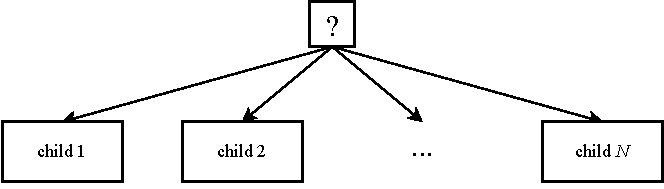
\includegraphics[width=0.75\textwidth]{figures/20_state_of_the_art/fallback.pdf}
    \caption{Graphical BT of a Fallback with \textit{N} childs}
    \label{fig:fallback}
\end{figure}
\lstset{language=C++, mathescape=true, caption={Algorithm of a Fallback with \textit{N} childs}, label={lst:pseudo_code_fallback}, morekeywords={from, to, is, do, then, end}}
\begin{lstlisting}[float=h]
for i from 1 to %\textit{N}% do:
  child_status $\gets$ tick(child[i])
  
  if child_status is %\textit{Running}% then:
      return %\textit{Running}%
      
  if child_status is %\textit{Success}% then:
      return %\textit{Success}%
end

return %\textit{Failure}%
\end{lstlisting}
A Fallback node (also known as a Selector), unlike the Sequence, executes only one child successfully. All children are updated from left to right, as shown in Figure \ref{fig:fallback} and Algorithm \ref{lst:pseudo_code_fallback}. If a child returns Success, the Fallback is completed. If a child returns Failure, the next child is started.

In addition to the Sequence and Fallback control nodes, there is also the Parallel node. In this structure, all children are started simultaneously, and the final state of the Parallel node is determined based on a comparison between a defined count M and the number of successfully completed children, as shown in Figure \ref{fig:parallel} and Algorithm \ref{lst:pseudo_code_parallel}.

\begin{figure}[h]
    \centering \captionsetup{justification=centering}
    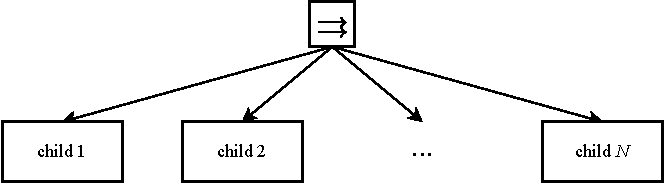
\includegraphics[width=0.75\textwidth]{figures/20_state_of_the_art/parallel.pdf}
    \caption{Graphical BT of a Parallel with \textit{N} childs}
    \label{fig:parallel}
\end{figure}
  
\lstset{language=C++, mathescape=true, caption={Algorithm of a Parallel with \textit{N} childs and success count \textit{M}}, label={lst:pseudo_code_parallel}, morekeywords={from, to, is, do, then, end}}
\begin{lstlisting}[float=!h]
for i from 1 to %\textit{N}% do:
    child_status[i] $\gets$ tick(child[i])
end
    
if success_count(child_status) >= %\textit{M}% then:
    return %\textit{Success}%
        
if failure_count(child_status) > (%\textit{N}% - %\textit{M}%) then:
    return %\textit{Failure}%

return %\textit{Running}%
\end{lstlisting}


\begin{table}[h]
\centering \captionsetup{justification=centering}
\resizebox{\textwidth}{!}{%
%\setlength{\extrarowheight}{8pt}
\begin{tabular}{lclll}
\toprule
\textbf{} & \multicolumn{1}{l}{\textbf{}} & \multicolumn{3}{c}{\textbf{Return Status}} \\ \midrule
\multicolumn{1}{c}{\textbf{Type}} & \textbf{Symbol} & \multicolumn{1}{c}{\textbf{Success}} & \multicolumn{1}{c}{\textbf{Failure}} & \multicolumn{1}{c}{\textbf{Running}} \\ \midrule
\textbf{Action} & Text & When completed & In case of errors & During execution \vspace{3mm}\\
\textbf{Condition} & Text & When condition is true & When condition is false & Never \vspace{3mm}\\
\textbf{Sequence} & $\to$ & When all children are \textit{Success} & When a child is \textit{Failure} & When a child is \textit{Running} \vspace{3mm}\\
\textbf{Fallback} & ? & When a child is \textit{Success} & When all children are \textit{Failure} & When a child is \textit{Running} \vspace{3mm}\\
\textbf{Parallel} & $\rightrightarrows$ & \begin{tabular}[c]{@{}l@{}}When $\ge$ \textit{M} \\ children are \textit{Success}\end{tabular} & \begin{tabular}[c]{@{}l@{}}When > \textit{N} - \textit{M} \\ children are \textit{Failure}\end{tabular} & \begin{tabular}[c]{@{}l@{}}As long as limits \\ are not reached\end{tabular} \vspace{3mm}\\
\textbf{Decorator} & $\diamond$ & Depending on the function & Depending on the function & Depending on the function \\ \bottomrule
\end{tabular}%
}
\caption{Overview of the elements of a Behavior Tree}
\label{tab:overview_bt}
\end{table}

An overview of the functions of each element is given in Table \ref{tab:overview_bt}. \Glspl{bt} are an evolution of \gls{fsm}, which are still widely used, but offer several advantages over them. The following are the advantages and disadvantages of \glspl{bt}. These characteristics are not necessarily unique to \glspl{bt}, but also apply to other concepts such as \glspl{hfsm} or decision trees \cite{colledanchise_behavior_2018}.

\begin{enumerate}
  \item \textbf{Modularity:} Individual subsystems can be modified and replaced as needed. The entire BT can also be reused as a module.
  \item \textbf{Hierarchical Structure:} Each control node introduces an additional level of hierarchy, making the overall behavior easier to understand.
  \item \textbf{Reusability:} Defined interfaces allow code to be used in multiple locations.
  \item \textbf{Reactiveness:} By continuously updating the BT, actions can be executed in a closed loop, enabling dynamic responses to the environment.
  \item \textbf{Intuitive Representation:} The graphical representation remains understandable even for complex systems.
  \item \textbf{Automatic Analysis:} Tools are available to monitor robustness and efficiency. BTs can also be created and monitored live using graphical editors.
  \item \textbf{Automatic Generation:} BTs can be generated during execution using machine learning techniques.
\end{enumerate}

However, there are also some disadvantages of BTs:

\begin{enumerate}
  \item \textbf{Complexity of the Engine:} Ensuring parallelism is necessary, but there are existing frameworks available to handle this.
  \item \textbf{Computational Intensity:} Updating all control nodes and conditions at each tick can be computationally intensive, potentially affecting real-time performance on weaker systems.
  \item \textbf{Implementation Overhead for Simple Behaviors:} For very short behaviors, direct programming or a simple FSM may be more efficient.
  \item \textbf{Immaturity of Behavior Trees:} Compared to widely adopted FSMs, there are fewer applications and software available for BTs.
\end{enumerate}

%% ==============================
\section{Hierarchical Path Planning}
\label{sec:hierarchical_planning}
%% ==============================
This section presents the related work in the area of path planning with hierarchical graphs. It gives an overview of the relevant existing work corresponding to the first research question: "How to navigate in complex multi-floor environments". 
A \Gls{h_graph} is a graph where each node in the graph holds a subgraph itself. This is used for hierarchical structuring of information, while the connections in a graph also represent information. The connections in a graph can be any configuration of non-directional, directional, bi-directional, sparse or densely connected. This depends on the data being stored. For navigation, this data may be the logical subdivisions of a complex environment such as a research campus. The hierarchical layers could be buildings, floors, rooms, and the gridmap itself. The structure of a \gls{h_graph} can be represented as a tree. A \gls{h_graph} with three hierarchical layers can be represented as a tree with a depth of three. An example of the structure of a \gls{h_graph} can be seen in Figure \ref{fig:h_graph}. Note that the internal connections of the nodes in each graph are not shown in the figure. 

\begin{figure}[h]
    \centering
    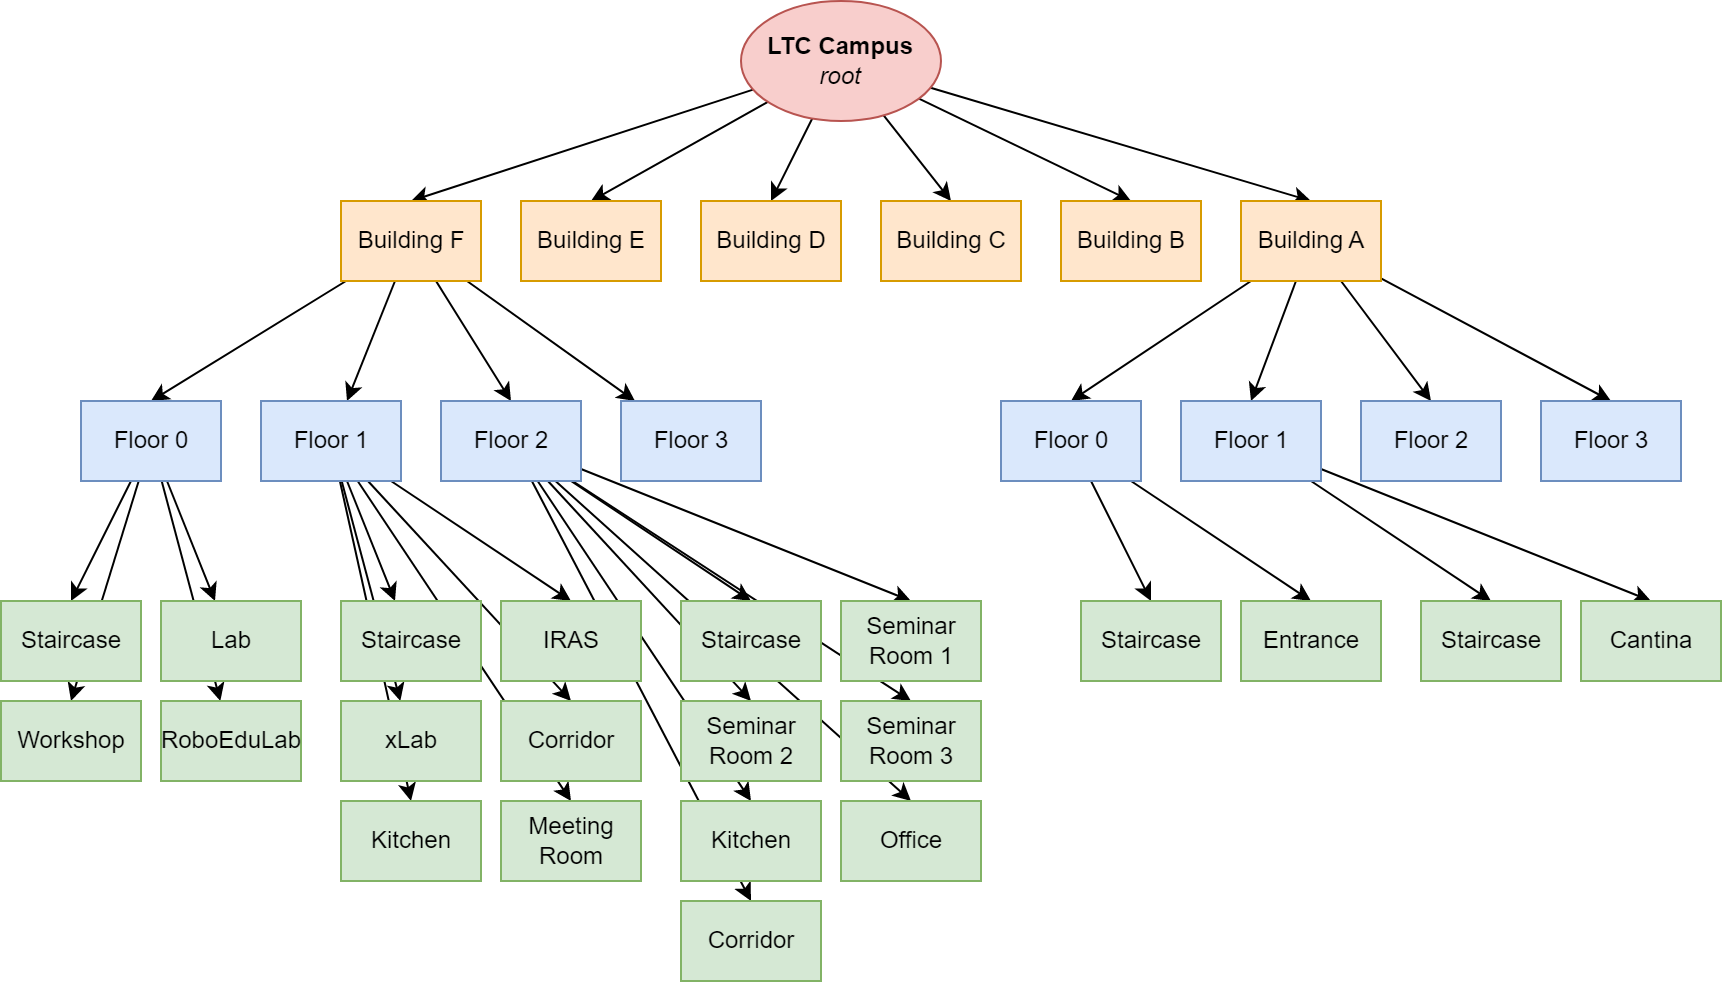
\includegraphics[width=\textwidth]{figures/20_state_of_the_art/hierarchical_graph.png}
    \caption[Representation of the structure of an H-Graph as tree]{Representation of the structure of an H-Graph with three hierarchical layers as a tree with depth three. This example shows the entire campus on layer 0 (red), the buildings of the campus on layer 1 (orange), the floors of each building on layer 2 (blue), and the individual rooms on layer 3 (green). For better clarity, only some sample nodes are fully expanded}
    \label{fig:h_graph}
\end{figure}

For use in navigation, the structure of the \gls{h_graph} represents the physical environment. This was first applied to mobile robot path planning by Fernandez and Gonzalez \cite{fernandez_hierarchical_1998} \cite{fernandez-madrigal_multi-hierarchical_2001}. The nodes in each graph are connected only if there is a drivable connection between these buildings or rooms. To make this space plannable, the connection has a cost corresponding to the shortest path distance between these two entities. This allows a common graph solver algorithm like Dijkstra or A* to find the shortest path in each graph. The advantage of a \gls{h_graph} is that not every leaf node in the tree has to be searched, because only the nodes that are on the path of the higher layer are relevant. This drastically reduces the search space and the time needed to find the optimal path in large environments. To combine a feasible path from all different graphs on the lowest layer, continuity between paths of different subgraphs must be ensured.

One proposed solution is the Hierarchical D* (HD*) algorithm by Cagigas \cite{cagigas_hierarchical_2005}. Cagigas breaks down an environment into a \gls{h_graph} by hierarchical decomposition. In each subgraph, the shortest connections to elevators are precalculated and stored as the weight of the connection in the metagraph. This is called materialization of costs. After finding the shortest path based on these costs, a reconstruction process is applied that connects the obtained partial paths. Cagigas extends the original D* algorithm \cite{hebert_optimal_1997} for this hierarchical planning. The D* algorithm is a dynamic or on-line version of the A* algorithm. The D* reuses and updates the computed cost from the initial search to replan the path when a dynamic obstacle blocks the initial path. This is an efficient way to replan without recalculating all the costs. Cagigas defines three types of hierarchical path planning: 
\begin{enumerate}
    \item \textbf{Horizontal Path Planning (HPP):} Paths between nodes connected in a horizontal way. Same as traditional robot path planning.
    \item \textbf{Vertical Path Planning (VPP):} Paths between nodes connected in a vertical way. Namely, paths that start on one floor and end on another floor of the same building.
    \item \textbf{Inter-building Path Planning (IPP):} Paths between nodes in different buildings. These paths start on a floor in one building and end on a floor in another building.
\end{enumerate}
Cagigas identifies the elevator selection problem shown in Figure \ref{fig:elevator_selection_problem}, which occurs in vertical path planning. The benefits of HD* cannot be applied here and a complete path replanning is required.

\begin{figure}[h]
    \centering
    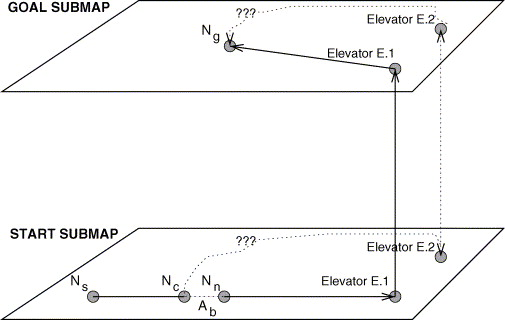
\includegraphics[width=0.75\textwidth]{figures/20_state_of_the_art/elevator_selection_problem.jpg}
    \caption[The elevator selection problem]{On-line vertical path planning. A “broken” arc \(A_b\) (obstacle) is detected between the current node \(N_c\) and the next node \(N_n\) in an initial path that joins a start node \(N_s\) and a goal node \(N_g\). The path planner module has to select an elevator entrance and there are two possibilities: the elevator entrance in the initial path (Elevator E.1) or an alternative elevator entrance (Elevator E.2). This last selection implies a complete path replanning. (Source: \cite{cagigas_hierarchical_2005})}
    \label{fig:elevator_selection_problem}
\end{figure}


Seder et al. \cite{seder_hierarchical_2011} proposed the Focussed Hierarchical D* (FHD*) algorithm. It improves the HD* algorithm by Cagigas in the following points:
\begin{enumerate}
\item Optimal placement of the bridge nodes needed to create the hierarchy.
    \item Focusing the search around the optimal path, which reduces the search area without losing optimality.
\item Introduction of partial starts and partial goals, which further reduce the computational time of replanning operations.
\end{enumerate}

In particular, the optimal placement of bridge points is important to ensure optimal paths across multiple hierarchies. Bridge nodes are placed along the optimal path to be followed by a mobile robot on its way from one room to another. Seder et al. calculate the optimal position by using a safety cost mask to find the middle point in a narrow passage. This corresponds to the safest point for a robot to pass through a door. Figure \ref{fig:bridge_node_placement} shows an example of bridge node placement. Seder et al. show that the FHD* algorithm is faster in replanning, requires fewer iterations, and explores fewer nodes than the D*, FD*, and HD* algorithms.

\begin{figure}[h]
    \centering
    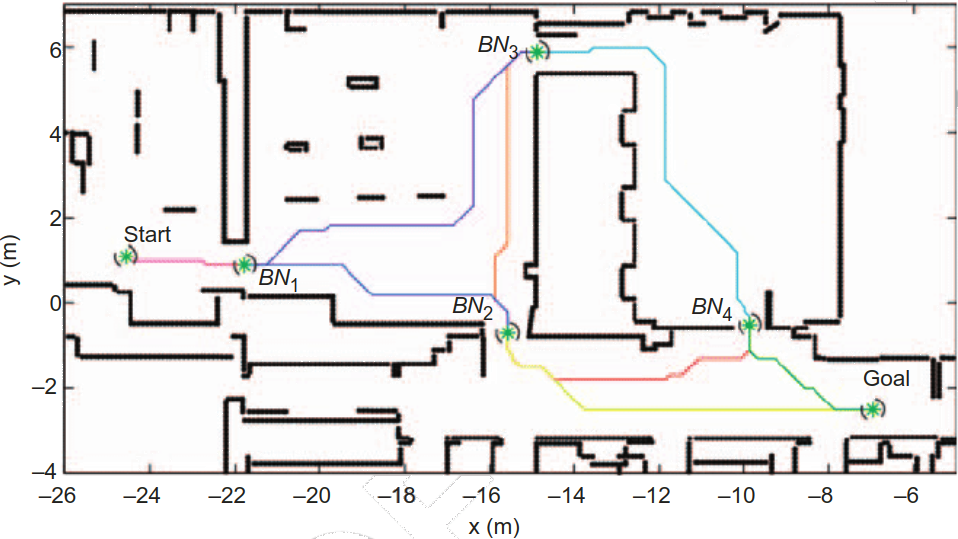
\includegraphics[width=0.75\textwidth]{figures/20_state_of_the_art/bridge_node_placement_paths.png}
    \caption[The bridge nodes with precalculated paths]{The bridge nodes BN 1-4 and the precalculated paths between them. (Source: \cite{seder_hierarchical_2011})}
    \label{fig:bridge_node_placement}
\end{figure}

Gregoric et al. \cite{gregoric_autonomous_2022} further extend the ideas of Seder et al. by using the E* algorithm \cite{philippsen_interpolated_2005}. This leverages A* to plan with an arbitrary angle instead of a fixed grid of 90 degrees (4 neighbors) or 45 degrees (8 neighbors). Gregoric et al. propose a method to automatically generate an H-Graph from CAD floor plans. At the floor plan level, this is done by using the safety cost mask. Connections between buildings are assumed to be at ground floor level. Vertical bridge connections are found with three conditions: 

\begin{enumerate}
    \item Comparing the positions of nodes on each floor
    \item The size of the room 
    \item The number of doors connecting this room to others
\end{enumerate}

Ryu \cite{ryu_hierarchical_2020} uses a different approach in generating the \gls{h_graph} as well as in finding the subpaths. Ryu uses only a two-layer hierarchy on a single floor. The two hierarchies are the so-called inter- and intra-regional graphs, which correspond to the connections between rooms and the path between the doors in each room. The hierarchy is created automatically by segmenting the entire floor plan into rooms. This is done using the marker-controlled watershed algorithm \cite{parvati_image_2009}. 

\begin{figure}[h]
    \centering
    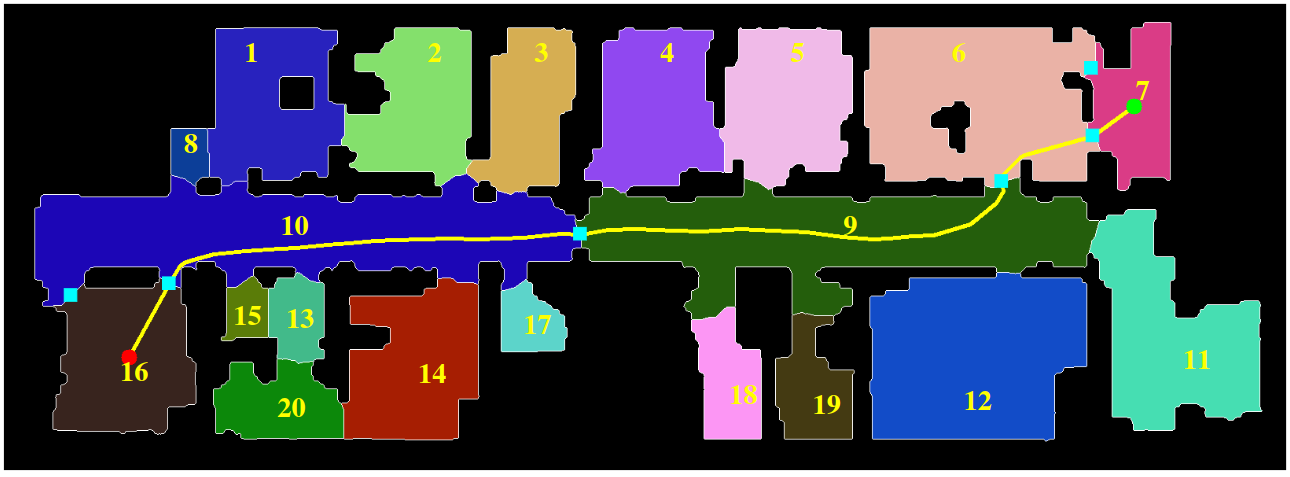
\includegraphics[width=0.75\textwidth]{figures/20_state_of_the_art/ryu_floor_path.png}
    \caption[The segmented floor map with combined inter-regional paths]{The segmented floor map with combined inter-regional paths (Source: \cite{ryu_hierarchical_2020})}
    \label{fig:ryu_floor_path}
\end{figure}

For the next step, Ryu proposes an algorithm for detecting safe junction nodes as a bridge between each room. A distance transform is used and the node with the highest distance to the obstacle is selected. This is similar to Seder et al. where a safety cost mask is applied. With these nodes, the intra-graph is created as shown in Figure \ref{fig:ryu_floor_path}. Ryu then uses a Skeletonization-Informed Rapidly Exploring Random Tree* (SIRRT*) to plan the inter-regional path. This is an extension of the classical sample-based RRT algorithm. It uses a skeletonized representation of the gridmap of a single room. This skeleton is used to inform the sampling of the RRT algorithm by generating nodes near the skeleton. Figure \ref{fig:ryu_sirrt} shows a solution path of SIRRT*. 

\begin{figure}[h]
    \centering
    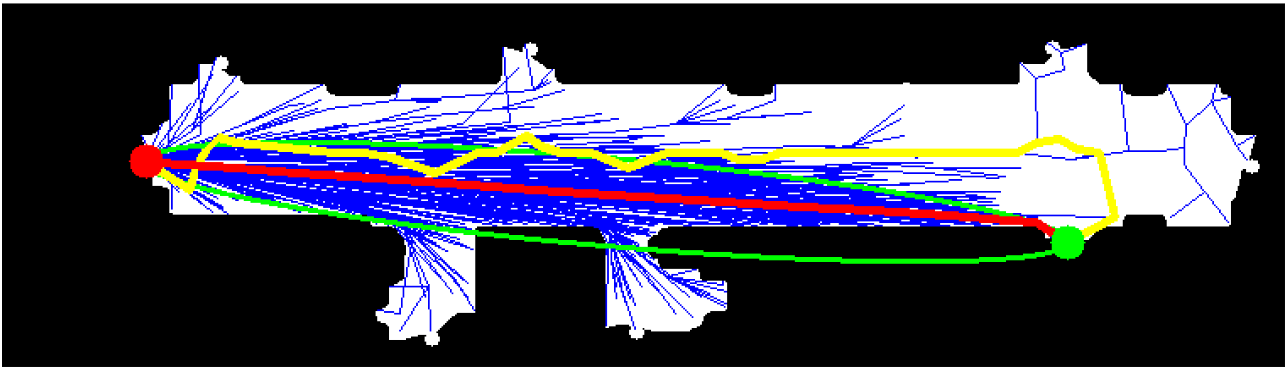
\includegraphics[width=0.75\textwidth]{figures/20_state_of_the_art/ryu_sirrt.png}
    \caption[Path planning with the SIRRT*]{An example of local path-planning for Segment “9” using the skeletonization informed rapidly exploring random tree* (SIRRT*): The red dot is the start position; the green dot is the goal. The initial skeleton path (yellow line). The final tree (blue line) and the optimized path (red line). The are for generating new sample nodes (green) (Source: \cite{ryu_hierarchical_2020})}
    \label{fig:ryu_sirrt}
\end{figure}

The previous papers used simulated 2D gridmap environments. They did not mention the application on a real robot. Dihman et al. \cite{dhiman_ros_2020} and Wang et al. \cite{wang_autonomous_2019} separately introduced a framework for using multi-floor navigation with ROS 1 on a real robot. Wang et al. use a modified A* algorithm to plan paths that are more centered in the corridor. The main contribution is the development of a convolutional neural network (CNN) to detect the current floor from images. A VGG16 network architecture is trained with 7,000 images to predict the robot's current floor. It is not mentioned whether automatic hierarchy generation or an H-graph is used for navigation. It is also not mentioned how the robot knows which elevator or floors to go to. Only on floor map level the path planning is done with the extended A*. Wang et al. use a real robot, the Pioneer 3-DX, and integrate everything into the existing ROS navigation stack. In comparison, Dihman et al. propose a method for global path planning on a cost graph. This is a single graph representing the floors and rooms of a single building, see Figure \ref{fig:dihman_cost_graph}. Vertical links are drawn in the same graph and represented with corresponding traversal costs. Dihman et al. also modify the existing ROS 1 navigation stack to support multiple robots and autonomous exploration. Additionally, the map server is extended for a multi-level occupancy gridmap and the global planner plans with respect to the cost graph.

\begin{figure}[h]
    \centering
    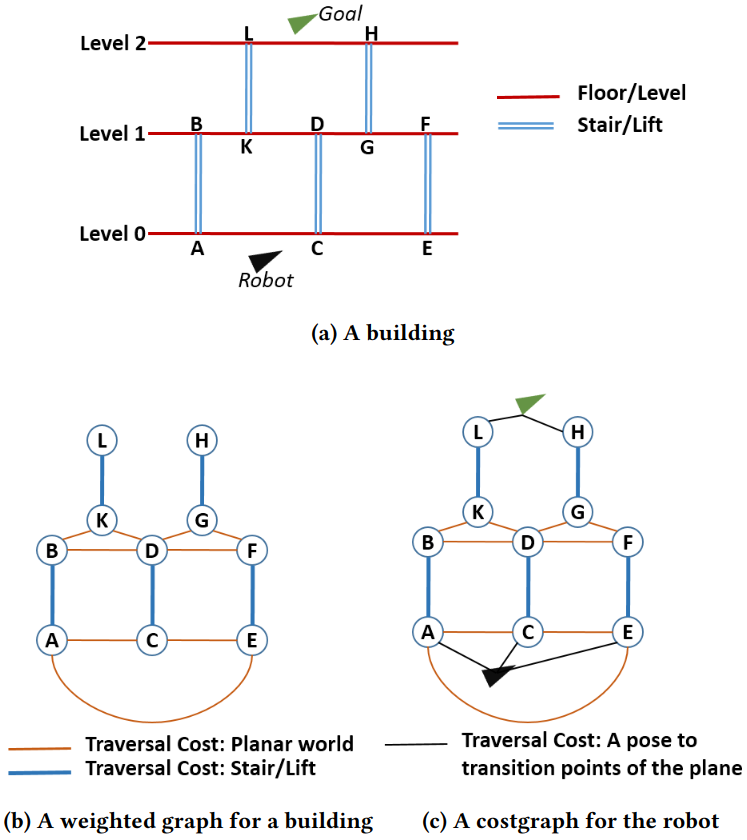
\includegraphics[width=0.75\textwidth]{figures/20_state_of_the_art/dihman_cost_graph.png}
    \caption[The cost graph for the robot]{(a) A building is represented as levels with stair or lift connection between floors, represented by thick blue parallel-lines. Blue and green color triangle represent current robot pose and goal pose respectively. (b) The building is transformed into a weighted graph. The node names refer to connection between the floor. (c) represents a weighted graph which includes edges from current robot pose and goal pose to the connection on the respective floor. This graph will be further used for solving global path planning. (Source: \cite{dhiman_ros_2020})}
    \label{fig:dihman_cost_graph}
\end{figure}

A comparison of these approaches to hierarchical path planning in multi-floor environments is done in Chapter \ref{sec:research_gap}. It can be seen that the focus is either on automatic hierarchy creation and efficient replanning or on integration with ROS and extension with additional features like CNN floor detection or multiple robots. This work aims to provide a mixture of these features by providing a method for automatic hierarchy creation for an H-Graph and integrating it in the new ROS 2 in simulation and for a real robot.

%% ==============================
\section{Straight Path Planning}
\label{sec:straight_paths}
%% ==============================
In this section, recent approaches to straight path planning are presented. This provides an overview of the relevant existing work that addresses the second research question: "How to plan paths that are straight and predictable?"

A common approach to path planning is to create a roadmap. The advantages of roadmaps are that they are very efficient for replanning because the roadmap is not recalculated each time. Depending on the creation process, roadmaps do not guarantee optimality, but they do provide a feasible answer within a short time. This is especially useful for motion planning in higher dimensional space for multi-axis manipulators. The configuration space \(C\) in 2D planar path planning has the same x and y axis as the real space. Obstacles in \(C\) space are inflated by the size of the robot to find collision free paths.

\begin{displayquote}
    \enquote{The roadmap approach to path planning consists of capturing the connectivity of the robot's free space in a network of one-dimensional curves, called the roadmap, lying in the free space \(C_{free}\) or its closure \(cl(C_{free})\). Once a roadmap \(R\) has been constructed . it is used as a set of standardized paths. Path planning is thus reduced to connecting the initial and goal configurations to points in \(R\) and searching \(R\) for a path between these points. The constructed path, if any, is the concatenation of three subpaths: a subpath connecting the initial configuration to the roadmap, a subpath contained in the roadmap, and a subpath connecting the roadmap to the goal configuration.} (Source: Latombe \cite{latombe_robot_2003})
\end{displayquote}

In the RRT or PRM algorithms presented earlier, the roadmap is created by randomly sampling free points in \(C\) space and connecting them with a collision-free edge. Another approach to creating a roadmap is the Voronoi diagram. The diagram is the set of all points with the greatest distance to neighboring obstacles. It consists of free paths which maximize the obstacle clearance, as seen in Figure \ref{fig:voronoi_diagram}
\begin{figure}[h]
    \centering
    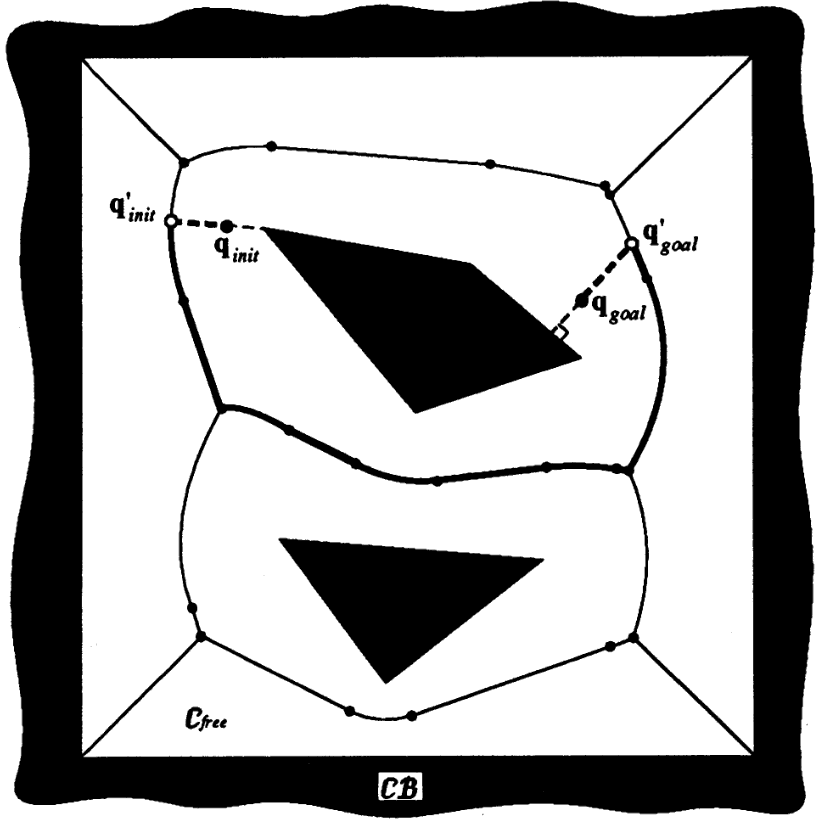
\includegraphics[width=0.5\textwidth]{figures/20_state_of_the_art/voronoi_diagram.png}
    \caption[The Voronoi diagram]{This figure shows the Voronoi diagram in a configuration space with a polygonal \(C\)-obstacle region. The free space is externally bounded by a rectangle. The initial and goal configurations \(q_{init}\) and \(q_{goal}\) are mapped into the Voronoi diagram to \(q'_{init}\) and \(q'_{goal}\), each by drawing the line along which its distance to the boundary to the \(C\)-obstacle region increases the fastest. (Source: \cite{latombe_robot_2003})}
    \label{fig:voronoi_diagram}
\end{figure}
\begin{figure}[b]
    \centering
    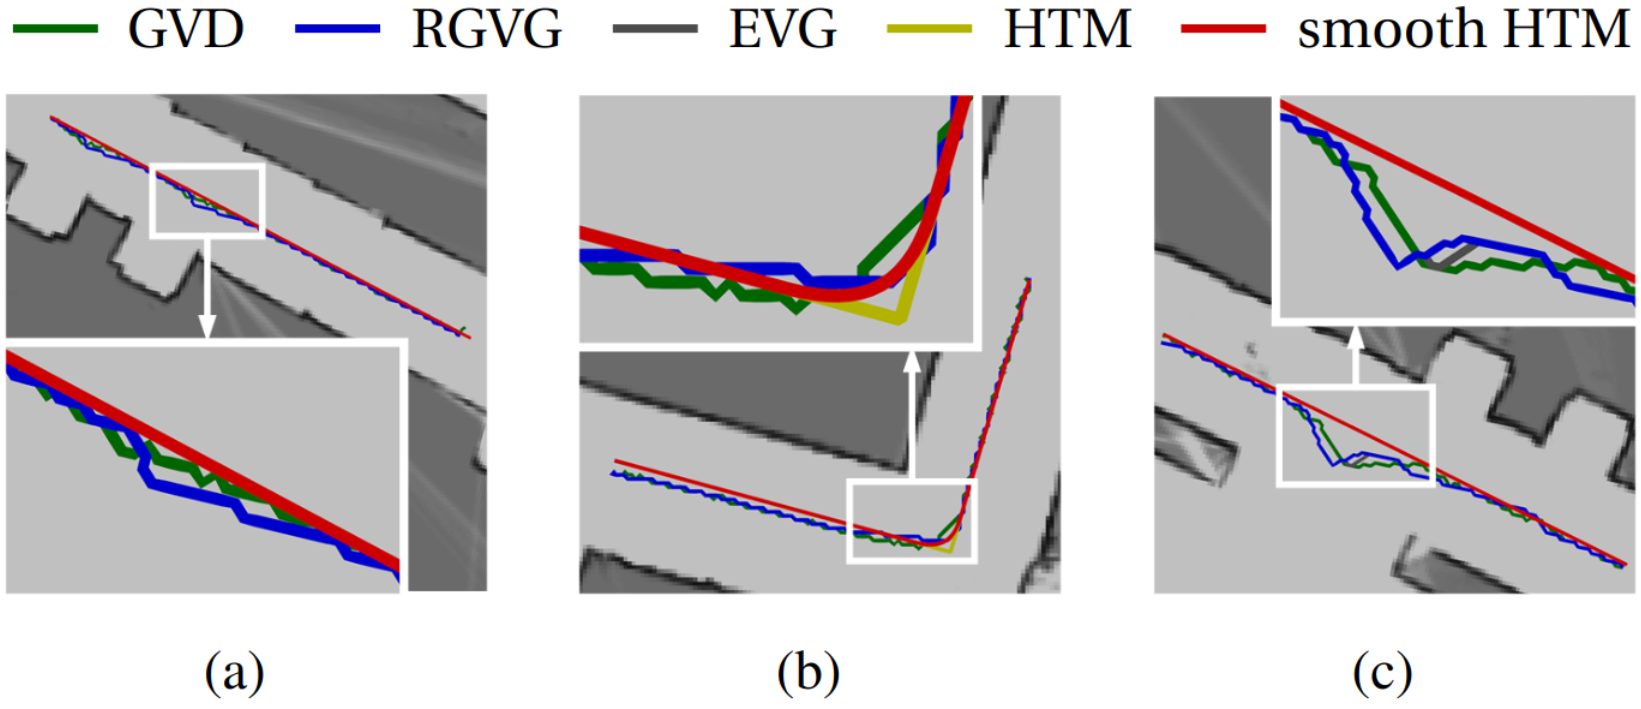
\includegraphics[width=0.75\textwidth]{figures/20_state_of_the_art/htm_path_comparison.png}
    \caption[Comparison between straight paths]{EVG based tracks coincide with RGVG based tracks within the sensory horizon. HTM based tracks coincide with smooth HTM when non-turning. (a) Tracks in the straight corridor. (b) Tracks in the turning corridor. (c) Tracks in the corridor with a room on the side. (Source: \cite{hou_straight_2021})}
    \label{fig:htm_path_comparison}
\end{figure}
The Generalized Voronoi Diagram (GVD), also called Voronoi Graph (GVG), is defined as the one-dimensional set of points equidistant from n or more obstacles in n dimensions. By pruning the graph based on a minimum length, the Reduced Generalized Voronoi Graph (RGVG) can be obtained. Beeson et al. \cite{beeson_towards_2005} extended the GVD to solve a limited sensory horizon of mobile robots. The Extended Voronoi Graph (EVG) changes from a center line in narrow corridors to a line following the walls in open spaces. However, the resulting paths suffer from noise in the measurements, resulting in non-straight paths. Also at intersections, the GVD and EVG produce paths that bend into the open space of the intersection. This creates an unnecessary curve for the straight direction as seen in Figure \ref{fig:htm_path_comparison} c).

Another approach to retrieve the topological map of an environment is the Straight Skeleton \cite{maurer_novel_1996}. Unlike Voronoi diagrams, this method does not use a distance function, but instead shrinks the obstacle polygon into free space. Each edge is moved along its normal axis at the same speed, creating a boundary where the shrunken edges touch. Based on this Straight Skeleton, Hou et al. \cite{hou_straight_2021} improved the straight path generation and countered the jitter problem of the EVG. Hou et al. propose the Hierarchical Topological Map (HTM) for the automatic generation of valid straight paths. The hierarchical approach first generates the straight skeleton and then detects intersections or small rooms where the jitter problem occurs. These sections are extracted and a separate skeleton is generated within them, which is then connected back to the global path. Finally, a clothoid-based smoothing method is applied to ensure curvature continuity of the generated tracks. A comparison of the discussed algorithms for generating topological maps and straight paths can be seen in Figure \ref{fig:htm_global_comparison}.

\begin{figure}[h]
    \centering
    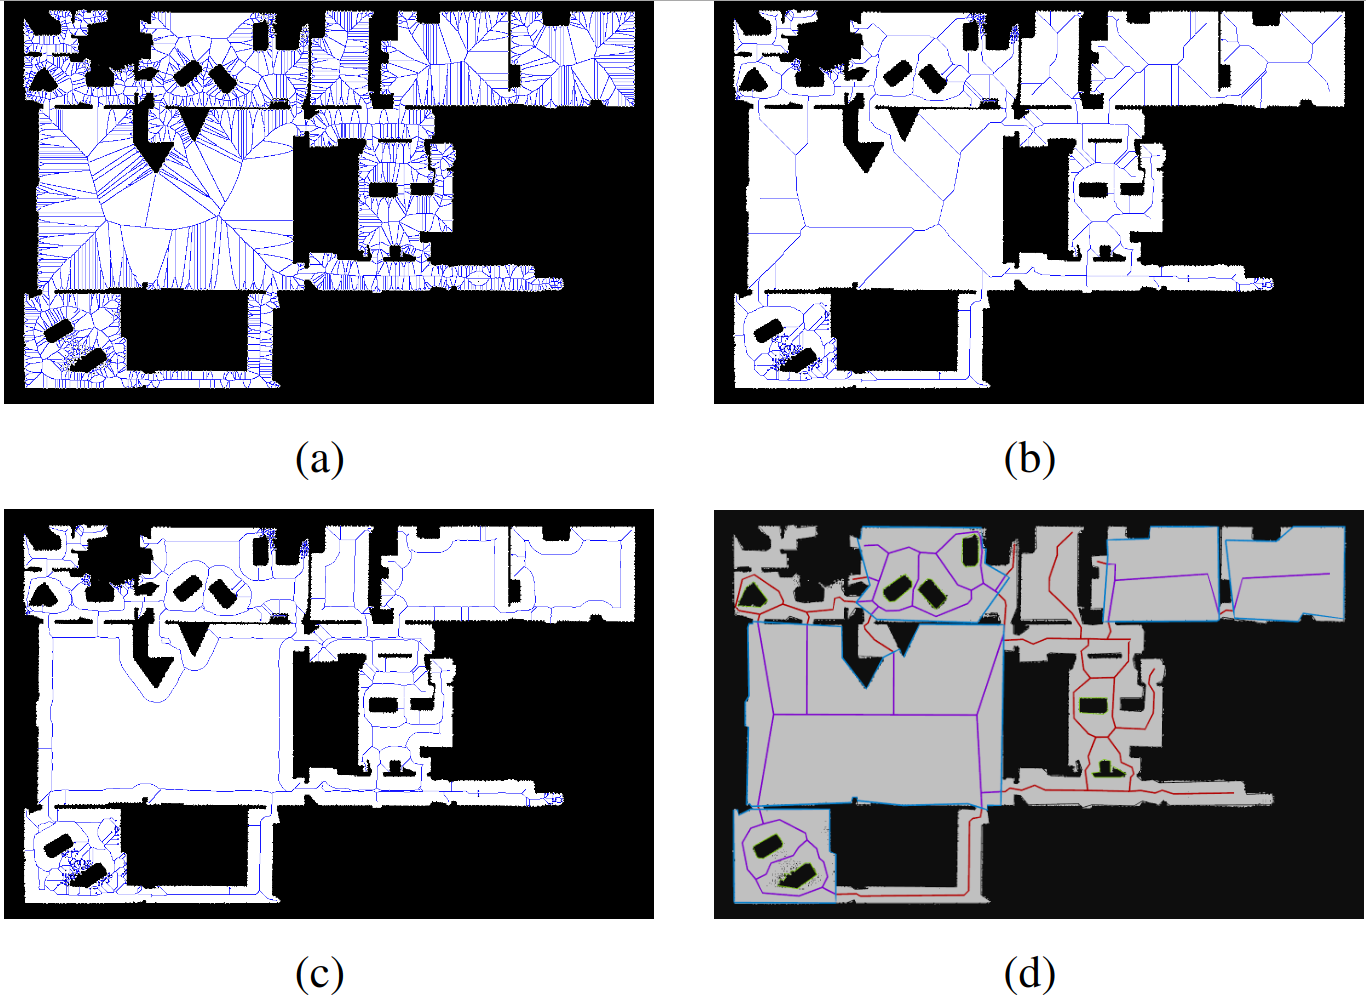
\includegraphics[width=\textwidth]{figures/20_state_of_the_art/htm_global_comparison.png}
    \caption[Comparison of generated topological maps]{Comparison of skeleton generation, using the gridmap obtained from \cite{beeson_towards_2005}. (a) GVD. (b) RGVG. (c) EVG with a sensory horizon of 1.25m. (d) HTM. Primary tracks, secondary tracks, and regions are marked in red, purple, and blue, respectively. (Source: \cite{hou_straight_2021})}
    \label{fig:htm_global_comparison}
\end{figure}

The presented methods focus on the goal of extracting a topological map from the gridmap. The HTM also focuses on generating paths that are straight. Further discussion on the limitations of these approaches and the resulting research gap that this work aims to address is given in Chapter \ref{sec:research_gap}. 

%% ==============================
\section{Research Gap}
\label{sec:research_gap}
%% ==============================
Table \ref{tab:overview_q1} gives an overview of the state of the art related to research question 1: "How to navigate in complex multi-floor environments? The different approaches to hierarchical path planning were presented in Chapter \ref{sec:hierarchical_planning}, this chapter discusses the limitations of these methods and shows the research gap for this work.

\begin{table}[h]
\centering \captionsetup{justification=centering}
\caption{Overview on the state of the art in hierarchical path planning}
\label{tab:overview_q1}
\resizebox{\textwidth}{!}{%
\begin{tabular}{@{}llllllll@{}}
\toprule
\textbf{Key topics} & \multicolumn{1}{c}{\textbf{\begin{tabular}[c]{@{}c@{}}Cagigas\\2005 \cite{cagigas_hierarchical_2005}\end{tabular}}} & \multicolumn{1}{c}{\textbf{\begin{tabular}[c]{@{}c@{}}Seder et al.\\2011 \cite{seder_hierarchical_2011}\end{tabular}}} & \multicolumn{1}{c}{\textbf{\begin{tabular}[c]{@{}c@{}}Gregoric et al.\\2022 \cite{gregoric_autonomous_2022}\end{tabular}}} & \multicolumn{1}{c}{\textbf{\begin{tabular}[c]{@{}c@{}}Ryu\\2020 \cite{ryu_hierarchical_2020}\end{tabular}}} & \multicolumn{1}{c}{\textbf{\begin{tabular}[c]{@{}c@{}}Wang et al.\\2019 \cite{wang_autonomous_2019}\end{tabular}}} & \multicolumn{1}{c}{\textbf{\begin{tabular}[c]{@{}c@{}}Dihman et al.\\2020 \cite{dhiman_ros_2020}\end{tabular}}} & \multicolumn{1}{c}{\textbf{\begin{tabular}[c]{@{}c@{}}{[}This work{]}\\2023\end{tabular}}} \\ \midrule
\begin{tabular}[c]{@{}l@{}}Path planning\\ algorithm\end{tabular} & HD* & FHD* & E* & SIRRT* & A*' & \begin{tabular}[c]{@{}l@{}}? /\\ Dijkstra\end{tabular} & \begin{tabular}[c]{@{}l@{}}ILIR /\\ Dijkstra\end{tabular} \\
\smallskip \\
\begin{tabular}[c]{@{}l@{}}Efficient on-line\\ replanning\end{tabular} & Yes & Yes & Yes & No & No & No & Yes \\
\smallskip \\
Map source & 2D Sim & 2D Sim & \begin{tabular}[c]{@{}l@{}}Floor\\ plans\end{tabular} & SLAM & SLAM & \begin{tabular}[c]{@{}l@{}}SLAM\\ Multi-robot\end{tabular} & SLAM \\
\begin{tabular}[c]{@{}l@{}}Hierarchy\\ creation\end{tabular} & Manual & \begin{tabular}[c]{@{}l@{}}Safety\\ cost mask\end{tabular} & \begin{tabular}[c]{@{}l@{}}Safety\\ cost mask,\\ matching\end{tabular} & \begin{tabular}[c]{@{}l@{}}Water-\\ shed\end{tabular} & \begin{tabular}[c]{@{}l@{}}CNN floor\\ detection\end{tabular} & Manual & Watershed \\
\smallskip \\
Hierarchy levels & 3 & 2 & 4+ & 2 & 3 & 3 & 4+ \\
\smallskip \\
\begin{tabular}[c]{@{}l@{}}Implementation\\ on real robot\end{tabular} & - & - & - & - & ROS 1 & ROS 1 & ROS 2 \\ \bottomrule
\end{tabular}%
}
\end{table}

The earlier work of Cagigas and Seder et al. focuses on solving the planning problem as a whole. They develop a single planner that solves the global path through the hierarchy as well as the path at the lowest gridmap level. In addition, they use a D* algorithm that is very efficient for replanning when obstacles are detected. This approach results from the fact that at this time there was no open source framework for path planning like ROS. As a result, most robotics problems had to be solved from scratch. With the wide distribution of ROS, there are many open source implementations for common planners. This has the advantage of benefiting from efficiently implemented planners in an integrated framework, and allowing one to focus on developing only the missing piece. This development can be seen in Wang et al. and Dihman et al., as both use ROS 1 and don't implement the basic planners themselves. The disadvantage is that a combined solution to the whole problem of hierarchy solving and path planning might be more efficient. However, reusability and community-defined interfaces allow rapid development in robotics research, and thus building on existing software is currently preferred. The analysis of the available literature shows that currently no such open source solution exists in ROS 2. The goal of this work is to develop a hierarchical path planner using the existing framework of ROS 2 and Nav2.

Gregoric et al. use the path planning ideas of Seder et al. and focus on automatically generating a hierarchical graph of the environment from floor plans. This extends the previous approaches as the number of levels is theoretically infinite. However, automatic hierarchy creation is only shown for room segmentation and floor matching. Additionally, a very simple multi-building environment is assumed, where vertical bridge nodes are always directly above each other and only connect floors of the same building. Other buildings are assumed to have only one connection between them on the ground floor. Although in more complex environments bridges on upper floors, ramps or densely connected building sections are possible. Ryu, on the other hand, focuses only on creating hierarchies for two levels, but proposes a new method for automatic room segmentation from SLAMed gridmaps. The goal of this work is to use the ideas of Gregoric et al. about n-level hierarchies for complex environments with arbitrary connections and to use the approach of Ryu for automatic room segmentation. Since neither work has been implemented on a real robot or is available as open source, the developed algorithms should be available for a real mobile robot with ROS 2.

For the straight path planning problem, a comparison of existing approaches can be seen in Figure \ref{fig:htm_global_comparison}. Only Hou et al. focus on straight path generation, the most common approach for a straight indoor roadmap is manual waypoint selection. A promising tool for this is OpenRMF from OpenRobotics \cite{openrobotics_open-rmf_2023}, which is currently under development. The goal of this tool is mainly fleet management and interoperability between robot vendors, but it also uses a roadmap of pre-planned straight paths. There are currently no plans to automatically generate these straight paths. For real production environments, this is due to safety reasons. However, having a tool that first proposes straight paths that can then be refined by manually moving specific waypoints, would drastically reduce the implementation time. The goal of this work is to develop such an algorithm for an initial straight roadmap.

The HTM approach of Hou et al. mostly generates paths that are straight. This makes these paths predictable for humans walking in the same area as the mobile robot. All these approaches are also deterministic. That is, given the same gridmap, these algorithms always produce the same output path. There is no probabilistic function involved that generates random points as in RRT or PRM. A deterministic path is also more predictable for humans, since the robot will always behave the same way. The advantage is that humans working in the same area can learn the paths of the mobile robot and can predict areas where a robot might drive through. This is useful for the hospital environment of the PeTRA use case. However, the paths generated by Hou et al. are not ideal for open spaces and large rooms, as shown in Figure \ref{fig:htm_global_comparison} d). Suppose this is a lobby or other large room where people might be waiting or walking between doors. The paths generated by the HTM are not intuitive. One would expect a robot to move in a straight path parallel to the wall, not in a triangular path that moves at an angle and then returns to the same wall. This requires a metric for the quality of the straight paths and to measure the effect of disturbing the public space used by other people. This work compares the proposed roadmap planner with other approaches and proposes a metric for the disturbance of public space.

In general, this research area is not very active. There are a few algorithms and limited proof-of-concept implementations, but there is a lack of a complete solution to the problem. In particular, a comprehensive benchmark environment for multi-floor scenarios is needed to test and compare methods with other researchers. In addition, hierarchy creation for a large, complex environment is a slow and manual process that is not yet fully solved. Both of these issues are beyond the scope of this work, but once solved could pave the way for easy deployment of large fleets of robots in a multi-floor building. Given the increasing number of tasks that can be automated with the advanced capabilities of AI and scene understanding, more and more service tasks could be performed by mobile robots.